    \vspace{0.5cm}

            \begin{definition}
                {Function}\(A,B\) are sets. Suppose \textit{f} is a relation from \(A\) to \(B\). The statement that \textit{f} is a \textit{function} means that if \((a,b_1),(a,b_2) \in f\), then \(b_1 = b_2\)

                We will write \(f(a) = b\) when \((a,b)\in f\).

            \end{definition}
    
            \textbf{Notes}: We'll say \(f\) is a \textit{mapping} from \(A\) to \(B\) if the domain of \textit{f} includes all of \(A\). \\
            \indent We are lazy with the language that defines a function. Consider \(f\colon \R \rightarrow \R\) defined by \(f(x) = \frac{1}{x}\). \\
            \indent When \(f\colon A \rightarrow B\), we expect the domain to be \(A\), but it may actually be a subset of \(A\). \\
            \indent Either case is fine as long as you know the answer to ``What is the actual domain?'' \\
            \indent Likewise, when \(f\colon A \rightarrow B\), we'll call \(B\) the co-domain of \textit{f} and the range is the set, \(\{b\in B \ | \ \exists a \in A \colon (a,b) \in f\}\). Two ``such-thats'' for this statement to be true. \\
            \indent Also note that by the definition is saying that if \(f\) is a function from \(A\) to \(B\), then for each \(a\in A\) there is at most one  \(b\in B\).

            \vspace{0.5cm}

            \begin{figure}[h]
                \centering
                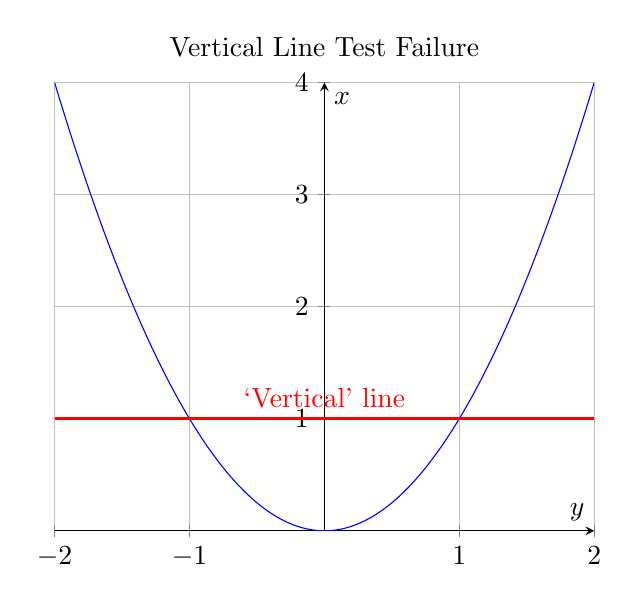
\begin{tikzpicture}
                \begin{axis}[
                    title={Vertical Line Test Failure},
                    xlabel={\(y\)},
                    ylabel={\(x\)},
                    axis lines=middle,
                    xmin=-2, xmax=2,
                    ymin=0, ymax=4,
                    grid=major,
                    xtick={-2,-1,...,2},
                    ytick={0,1,...,4},
                    domain=-2:2,
                    samples=100,
                ]
                % Plot the function for the 1st and 4th quadrants
                \addplot+[mark=none, blue] {x^2};
                
                % Add a horizontal line that goes through the parabola
                \draw [red, very thick] (axis cs:-2,1) -- (axis cs:2,1) node[pos=0.5, above] {`Vertical' line};
                \end{axis}
                \end{tikzpicture}
                \caption{Plot of Quadrants I and IV with \(x = y^2\)}
            \end{figure}


            

    
            \begin{definition}
                {Injective}Suppose \(f\colon A \rightarrow B\) is a function. The statement \textit{f} is \textit{one-to-one} (1-1) or \textit{injective}. This means that \((a_1,b), (a_2,b) \in f\), then \(a_1 = a_2\).
            \end{definition}

            \textbf{Think}: This can be rephrased as: if \(f(a_1) = b\) and \(f(a_2) = b\), then \(a_1 = a_2\). Or another common way might be \(f(a_1) = f(a_2) = b\).

        \section{Problems}

% ------------------------------------------------------------------------------
% Problem 43
% ------------------------------------------------------------------------------

            \begin{exercise}
                {Denial of Injective}Write the denial of \(f\) being injective.
            \end{exercise}
    
            \sol{
                The denial of \(f\) being injective means that there exists at least one pair of distinct elements \(a_1,a_2\in A\) (where \(A\) is the domain of \(f\)) such that \(f(a_1) = f(a_2) = b\) for some \(b\in B\) (where \(B\) is the co-domain of \(f\)). \\
                
                Therefore, the denial of the statement explicitly states the existence of two distinct inputs that yield the same output under \(f\). 
            }

% ------------------------------------------------------------------------------
% Problem 44
% ------------------------------------------------------------------------------
    
            \begin{exercise}
                {Injectivity}Suppose \(f\colon A\rightarrow B\) is a function, Then, \[f^{-1} \text{ is a function} \iff f \text{ is injective.}\]
            \end{exercise}
    
            \expf{
                (\(\Rightarrow\)) \\
                Assume \(f^{-1}\) is a function. To show \(f\) is injective, we must show that \(f\) has elements \((a_1,b), (a_2,b) \in f\) where \(a_1 = a_2\). We can do this by utilizing the fact that both \(f^{-1}\) and \(f\) are functions. Then, by rearranging the terms in the definition of function, we can show that \(f\) is indeed, one-to-one. \\
                
                Since \(f^{-1}\) is a function, we can assume its inverse, \(f\) is also a function. Then, because \(f\) is a function, we know that there are distinct \(a_1,a_2\) for which \(f(a_1) = f(a_2) = b\). And by the definition of the inverse relation, \((b,a_2),(b,a_1)\in f^{-1}\). Since \(f^{-1}\) is a function, then \(a_1 = a_2\). \\
                
                \indent Therefore, \(f\) must be injective by definition. \\

                \noindent\textit{Proof.} (\(\Leftarrow)\) \\
                Assume \(f\) is injective. To show that \(f^{-1}\) is a function, we must ensure that for each \(b\in B\) there is at most one \(a\in A\) such that \(f^{-1}(b) =a\) whenever \(f(a) = b\). \\

                By definition of injectivity, we have \(a_1 = a_2\) for any \(b\in B\) with \(f(a_1) = f(a_2) = b\). This guarantees a injective relation between the elements in \(A\) and \(B\). \\

                However, to show that \(f^{-1}\) is not only a relation, but also a function, we must begin by defining \(f^{-1}\). Since \(f\) is a a function, and thereby a relation, we can denote \(f^{-1}\) as the inverse relation. Hence, the definition of the inverse relation with substituted values is \(f^{-1} = \{(b,a)\in B\times A \colon (a,b) \in f\}\). \\

                Now, to show that \(f^{-1}\) is a function, we need to show that for every \(b\in B\), there exists a unique \(a\in A\) such that \(f^{-1}(b) = a\). Because \(f\) is injective, no two different \(a\)'s \(\in A\) map to the same \(b\in B\). Thereby reversing the direction from \(A\rightarrow B\) to \(B\rightarrow A\). This inherently ensures the existence of at most one \(a\) for each \(b\), which is exactly the definition of a function if \(B\rightarrow A\).\\

                Therefore, \(f^{-1}\) not only exists, but is also a function that maps each \(b\in B\) to a unique \(a\in A\).
            }

            \begin{definition}
                {Composition}Suppose \(f\colon A \rightarrow B\), and \(g\colon B\rightarrow C\) are functions. Then, we define the \textit{composition} of \textit{f} and \textit{g}, denoted \(g\circ f\) by \(\{(a,c, \in A\times C \ | \ \exists b\in B \colon (a,b)\in f)\) and \((b,c) \in g\}\).
            \end{definition}

            \begin{example}
                \(f \colon \R \rightarrow \R\) defined by \(f(x) = x^2\), and \(g \colon \R \rightarrow \C\) defined by \(g(x) = x + x^3i\). 
            \end{example}
            Then, \((3,9) \in f\) and \((9,9 + 9^3i) \in g\) implies \((3,9 + 9^3i \in g \circ f\)). But \((2,4)\in f\) and \((2,2 + 8i) \in g\) do not imply that \((2,2+8i)\in g\circ f\). \\

        \section{Problems}        

% ------------------------------------------------------------------------------
% Problem 45
% ------------------------------------------------------------------------------

            \begin{exercise}
                {Composition I}Suppose \(f\colon A \rightarrow B\) and \(g\colon B \rightarrow C\) are functions. Then, \[g\circ f \text{ is a function}.\]
            \end{exercise}

            \expf{
                Assume \(f\colon A \rightarrow B\) and \(g\colon B \rightarrow C\). To prove that \(g\circ f\) is a function, we need to show that for every \(a\in A\), there exists a unique \(c\in C\) such that \((g\circ f)(a) = c\). \\

                Suppose \(a\in A\). Since \(f\) is a function from \(A\rightarrow B\), for this \(a\), there exists a unique \(b\in B\) such that \(f(a)=b\). Similarly, given that \(g\) is a function from \(B \rightarrow C\), for that unique \(b\in B\), there exists a unique \(c\in C\) such that \(g(b) =c\). Therefore, for the chosen \(a\), \((g\circ f)(a) = g(f(a)) =g(b) = c\). This shows \(g(f(a))\) exists for all \(a\in A\).  
            }

% ------------------------------------------------------------------------------
% Problem 46
% ------------------------------------------------------------------------------

            \begin{exercise}
                {Composition II}Suppose \(f\colon A \rightarrow B\) and \(g\colon B\rightarrow C\) are injective. Then, \[g\circ f \text{ is injective.}\]
            \end{exercise}

            \expf{
                Assume \(f\) and \(g\) are injective. To prove that \(g\circ f\) is injective, we need to show that if \(g(f(x_1)) =g(f(x_2))\), then \(x_1 = x_2\), for \(x_1,x_2\in A\). \\
                
                \noindent Also assume that \(g(f(x_1)) = g(f(x_2))\). Since \(g\) is injective, then by definition, \(g(b_1) = g(b_2)\) implies \(b_1 = b_2\) for \(b_1,b_2\in B\). Then, applying this to our assumption, we get \(f(x_1) = f(x_2)\). Similarly, since \(f\) is injective, then \(f(x_1) = f(x_2)\) implies \(x_1 = x_2\) for \(x_1,x_2\in A\). \\
                
                Therefore, \(g\circ f\) is injective. 
            }


            \begin{definition}
                {Surjective}Suppose \(f\colon A \rightarrow B\) is a function. The statement that \(f\) is \textit{onto} or \textit{surjective} means that if \(b\in B\), then there exists an \(a\in A\) with \((a,b)\in f\).
            \end{definition}
            \textbf{Note}: Thus, a function is surjective if the range is the entire co-domain.


            \begin{definition}
                {Bijection}Suppose \(f\colon A \rightarrow B\) is a function (with domain consisting all of \(A\)). If \(f\) is both injective and surjective, we say that \(f\) is a \textit{bijection}.
            \end{definition}
            \textbf{Note}: \(f\colon A\rightarrow B\) is a bijection means: 
            \begin{itemize}
                \item \(f\) is a function (each \(a\) only maps to one \(b\)).
                \item \(\text{Domain } = A\)
                \item Injective (each \(b\) is mapped to by only one \(a\)).
                \item Surjective (\(\text{range } = B\))
            \end{itemize}

% ------------------------------------------------------------------------------
\newpage
% ------------------------------------------------------------------------------

        \section{Problems}

% ------------------------------------------------------------------------------
% Problem 47
% ------------------------------------------------------------------------------

            \begin{exercise}
                {Bijection I}Suppose \(f\colon A \rightarrow B\) is a  bijection. Then, \[f^{-1} \colon B \rightarrow A \text{ is a bijection.}\]
            \end{exercise}

            \expf{
                Assume that \(f\colon A \rightarrow B\) is bijective, meaning it is a function, its domain is all of \(A\), and it is both injective and surjective. To prove that \(f^{-1}\) is also bijective, we must show that \(f^{-1}\) is a function, its domain is all of \(B\), and that it is injective and surjective.
                \begin{enumerate}
                    \item \textbf{Function}: \\
                    Because \(f\) is injective, we know that by Problem 44, \(f^{-1}\) is a function.
                    
                    \item \textbf{Domain (All of \(B\))}: \\
                    Consider any element \(b \in B\). Given \(f\)'s surjectivity, there exists at least one \(a\in A\) such that \(f(a) =b\). By the definition of inverse relation, this relationship directly translates to \(f^{-1}(b) = a\) for all \(b\in B\). Thus showing that \(f^{-1}\)'s domain spans all of \(B\).
                    
                    \item \textbf{Injectivity}: \\ 
                    Suppose \(f^{-1}(b_1) = a\) and \(f^{-1}(b_2) = a\) for some \(b_1, b_2 \in B\). By the definition of inverse relation, \(f(a) = b_1\) and \(f(a) = b_2\). Then, \(b_1 = b_2\) because \(f\) is injective. Thus, \(f^{-1}\) maps distinct elements of \(B\) to distinct elements of \(A\), making \(f^{-1}\) injective. 
                    
                    \item \textbf{Surjectivity}: \\
                    \(f^{-1}\) is surjective when for all \(a\in A\), there is some \(b\in B\) such that \(f^{-1}(b) = a\). Since \(f\) covers all of \(A\), for any \(a\) there is a \(b\in B\) such that \(f(a) = b\). By the definition of inverse relation, this means \(f^{-1}(b) = a\) for every \(a\), making \(f^{-1}\) surjective.
                \end{enumerate}
                Therefore, because we have shown that \(f^{-1}\) is a function, its domain is all of \(B\), and it is both injective and surjective, it is a bijection.
            }
        
% ------------------------------------------------------------------------------
% Problem 48
% ------------------------------------------------------------------------------

            \begin{exercise}
                {Bijection II}Suppose \(f\colon A \rightarrow B\) and \(g\colon B \rightarrow C\) are both bijections. Then, \[g\circ f \text{ is also a bijection.}\]
            \end{exercise}

            \expf{
                Suppose \(f\colon A \rightarrow B\) and \(g\colon B\rightarrow C\) are both bijections. To show that \(g\circ f\) is also a bijection, we need to show that it is a function, its domain is all of \(A\), and it is surjective and injective. Because we have already shown that \(g\circ f\) is a function and injective by Problem 45 and Problem 46 respectively, we only need to show that \(g\circ f\) is surjective, and its domain is all of \(A\).
                \begin{enumerate}
                    \item \textbf{Function}: \\
                    By Problem 45, because \(f\) and \(g\) are functions, \(g\circ f\) is also a function.
                    
                    \item \textbf{Domain (All of \(A\))}: \\
                    For every \(a\in A\), \(f\) maps \(a\) to some \(b \in B\), and \(g\) maps to that \(b\) to some \(c \in C\). Hence every \(a\in A\) is mapped to some \(c\in C\) by \(g\circ f\). Thus showing that the domain of \(g \circ f\) is all of \(A\).
                    
                    \item \textbf{Injectivity}: \\ 
                    By Problem 46, because \(f\) and \(g\) are injective, \(g\circ f\) is also injective.
                    
                    \item \textbf{Surjectivity}: \\
                    Consider any \(c \in C\). Since \(g\) is surjective, there exists a \(b\in B\) such that \(g(b) = c\). Furthermore, because \(f\) is surjective, there exists an \(a \in A\) such that \(f(a) = b\). Therefore, \(g(f(a)) = c\), showing that for every \(c\in C\), there is an \(a\in A\) such that \(g \circ f(a) = c\), making \(g \circ f\) surjective.
                    
                \end{enumerate}
                Therefore, because we have shown that \(g\circ f\) is a function, its domain is all of \(A\), and it is both injective and surjective, it is a bijection.
            }


            \begin{definition}
                {Image}Suppose \(R\colon A \rightarrow B\). For relations, we define the \textit{image} of \(C\) under \(R\) as \(R(C) = \{b\in B\colon (c,b) \in R\) for some \(c\in C\}\). \\
                
                Suppose \(f\colon A \rightarrow B\). For functions, we define the \textit{image} of \(C\) under \(f\) as \(f(C) = \{b\in B\colon f(c) = b\) for some \(c\in C\}\). \\
            \end{definition}

            \textbf{Think}: \(f(C) \subseteq B\) vs. \(f(c) \in B\) for \(c\in C\). \\

        \section{Problems}

% ------------------------------------------------------------------------------
% Problem 49
% ------------------------------------------------------------------------------

            \begin{exercise}
                {}Suppose \(f\colon A\rightarrow B\) is a function with \(A\) being the domain of \(f\). Then, \[f \text{ is injective } \iff \text{ for any } C\subseteq A, f^{-1}(f(C)) = C\]
            \end{exercise}

            \expf{
                (\(\Rightarrow\)) \\
                
                \noindent (\(\subseteq\))\\
                \indent Let \(x\in f^{-1}(f(C))\). By the definition of image of \(f(C)\), we know that there exists a \(b \in f(C)\) such that \((b,x) \in f^{-1}\). Then, by definition of image under \(f\), \(b\in f(C)\) implies that there exists a \(c\in C\) such that \(f(c) = b\).\\
                
                \noindent Now, since \((b,x) \in f^{-1}\), by the definition of the inverse relation, this means \(f(x) = b\). Given that \(f\) is injective, it must be the case that \(x = c\). Hence, \(x\in C\) and \(f^{-1}(f(C)) \subseteq C\). \\

                \noindent (\(\supseteq\)) \\
                \indent Let \(c\in C \subseteq A\). That is, \(c\) is contained in the set \(C\) which is a subset of \(A\), which is defined as the domain of \(f\). By definition of image, we know there must exist some \(x\) such that \(x = f(c) \in B\). Then, by definition of inverse relation, we know that \((x,c) \in f^{-1}\). Thus, \(c \in f^{-1}(f(C))\) by the definition of image. \\
            
                Therefore, since \(f\) is injective and because \(f^{-1}(f(C)) \subseteq C\) and \(C\subseteq f^{-1}(f(C))\), for any \(C \subseteq A\), then \(f^{-1}(f(C)) = C\) by Theorem 1. \\

                \noindent\textit{Proof}. (\(\Leftarrow\)) \\
                \indent Suppose for all \(C \subseteq A, f^{-1}(f(C)) = C\). Then, for some \(a_1,a_2\in A\), let \(f(a_1) = f(a_2) = b\) by definition of function. We want to show that if \(f(a_1) = f(a_2)\), then \(a_1 = a_2\).  \\
                
                \noindent Consider the set \(C = \{a_1,a_2\} \subseteq A\). Since \(f(a_1) = f(a_2)\), both \(a_1\) and \(a_2\) are mapped to the same element \(b \in B\). Therefore, \(f(C)\), which is the image of \(C\) under \(f\), contains the element \(b\) by definition. Thus, the pre-image of the image of \(C\), \(f^{-1}(f(C))\), must include both \(a_1\) and \(a_2\), since both are mapped to \(b\). \\

                \noindent Then, since \(C = \{a_1, a_2\}\), and \(f^{-1}(f(C)) = C\), then we can substitute \(C\) for \(\{a_1,a_2\}\) to get \(f^{-1}(f(\{a_1,a_2\})) = \{a_1,a_2\}\). By the given information, we know that the operation of \(f^{-1}\) on \(f\) yields precisely the original set. Thus, \(a_1\) and \(a_2\) must be the same because if they weren't, \(f^{-1}(f(C))\) would not precisely equal the original set, \(C\). \\

                \noindent Therefore, we have shown that \(f(a_1) = f(a_2)\), implies \(a_1 = a_2\), and hence, \(f\) is injective by definition. 
            }
% \Leftarrow \\
% For all C \in A, f^{-1}(f(C)) = C

% Let (a_1,b),(a_2,b)\in f 
% Consider C = {a_1}
%... a_1 = a_2

% ------------------------------------------------------------------------------
% Problem 50
% ------------------------------------------------------------------------------

            \begin{exercise}
                {}Suppose \(f\colon A\rightarrow B\) is a function. Then, \[f \text{ is surjective } \iff \text{ for any } D\subseteq B, f(f^{-1}(D)) = D\]
            \end{exercise}

            \expf{
                (\(\Rightarrow\)) \\
                
                \noindent (\(\subseteq\))\\
                \indent Let \(x\in f(f^{-1}(D))\). By the definition of image, we know there exists a \(c \in f^{-1}(D)\), and thus \(f(c) = x\) by definition of inverse relation. 
                
                \noindent Now, let \(y \in D\) such that \((y,c) \in f^{-1}\). By the definition of \(f^{-1}\), \(f(c) = y\). Then, because \(f\) is a function, \(x\) must equal \(y\), and thereby since \(y \in D\), \(x \in D\). \\

                \noindent (\(\supseteq\)) \\
                \indent Let \(d\in D\). By the definition of image, we know there is an element \(q\) such that \((d,q) \in f^{-1}\). Therefore, we know \(q\) has to be in the image of \(D\) by definition. Thus, \(q \in f^{-1}(D)\). Then, there must exist some \(p \in f(f^{-1}(D))\) such that \(p = f(q)\) by definition of image. Thus, by definition of \(f^{-1}\), \(f(q) = d\), and thereby, \(d = p\), and by substitution, \(d \in D\), so \(D \subseteq f(f^{-1}(D))\). \\

                Therefore, because \(D \subseteq f(f^{-1}(D))\) and \(f(f^{-1}(D)) \subseteq D\), by Theorem 1, \(D = f(f^{-1}(D))\). \\

                \noindent\textit{Proof}. (\(\Leftarrow\)) \\
                \indent Suppose for all \(D \subseteq B\), \(f(f^{-1}(D)) = D\). We must show that \(f\) maps surjectively to every element of \(B\). \\

                \noindent Consider the set \(D = \{b\}\). We know that \(f^{-1}(D)\) represents the pre-image of \(D\); meaning it including all elements \(a\in A\) for which \(f(a) \in D\). Given \(D = \{b\}\), this translates to all \(a\in A\), \(f(a) = b\). \\
                
                \noindent Then, by using substitution, we can see that \(f(f^{-1}(\{b\}) = \{b\}\). This equation implies that the image under \(f\) of the pre-image of \({b}\) is exactly \({b}\). Thus, because \(f(f^{-1}(\{b\})) = \{b\}\), we know at least one element in \(A\) maps to \(b\). \\

                \noindent Therefore, since every element \(b\in B\) is the image of some element in \(A\), we've shown that \(f\) is surjective by definition.
            }


        \begin{definition}
            {Immediate Successor}Suppose \(A\) is a set. We define the \textit{immediate successor} of \(A\) to be the set \(A^+ = A \cup \{A\}\).
        \end{definition}

        \section{Problem}

% ------------------------------------------------------------------------------
% Problem 51
% ------------------------------------------------------------------------------

            \begin{exercise}
                Suppose \(A\) is a set. Then, \[A^+ \ne \emptyset\]
            \end{exercise}

            \expf{
                Suppose \(A\) is a set. \\

                \noindent Since \(A^+\) is the union of \(A\) and the set of \(A\), \(A^+\) contains at least one element, \(\{A\}\). Therefore, by the negation of Problem 11, \(A^+ \ne \emptyset\).
            }


            \begin{definition}
                {Successor Set}Suppose that \(A\) is a set. The statement that \(A\) is a \textit{successor set} means that \begin{enumerate}
                    \item \(\emptyset \in A\) and 
                    \item if \(a\in A\), then \(a^+ \in A\)
                \end{enumerate}
            \end{definition}

            \textbf{Think}: \(A\) successor set then, \(\emptyset \in A, \emptyset^+\in A, (\emptyset^+)^+\in A \dots\)

    